\documentclass[10pt,a4paper,final,twoside,openany,article]{memoir}
% [12pt, 11pt, landscape, titlepage, a4paper, draft, twoside, oneside, 
%  openleft, openright, openany]

\chapterstyle{hangnum}

%BASIC PACKAGES
\usepackage{eso-pic,fix-cm,ae,aecompl,ifthen}         
\usepackage[danish,english]{babel} % last language decides document language!
\usepackage[utf8x]{inputenc}          %text encoding
\usepackage{amsmath,amssymb, amsbsy}  % math
\usepackage{graphicx}
\usepackage[usenames,dvipsnames]{color}
\usepackage[british]{isodate}
%\usepackage{morefloats}

\newsubfloat{figure}

%MISC. PACKAGES
%\usepackage{multicol}        % \begin{multicols}{2} \end{multicols}
%\usepackage{array}           % advanced tables
%\usepackage{multirow}        % advanced tables
%\usepackage{longtable}       % split tables over pages
%\usepackage{textcomp}        % symbols
%\usepackage{verbatim}        % monospace code environment
%\usepackage{pdflscape}       % \begin{landscape} \end{landscape}
%\usepackage{semantic}        % Good for proof trees and math ligatures
%\usepackage[noend]{algorithmic}
\usepackage{microtype}        % AWESOME typography!
\usepackage{colortbl}
\usepackage{marvosym}
%Kan bruges som \fixme{blabla}. Vises sålænge tex doc er i draft.
\usepackage[draft] { fixme } 


%FONT
\usepackage[T1]{fontenc}
\usepackage{palatino}              % font : garamond
\linespread{1.05}                  % Palatino needs more leading (space between lines)
\usepackage{bera}
%\renewcommand{\ttdefault}{cmtt}    % alternative monospace font
%\renewcommand{\rmdefault}{ugm}
\usepackage[sc]{mathpazo}
%\usepackage{euler}                % weirdo math
%PAGE DIMENSIONS

%\usepackage[left=4.5cm, right=4.5cm, top=4.4cm, bottom=4.5cm]{geometry}


%HEADERS
\makepagestyle{myheadings}

%\makepsmarks{myheadings}{
%  \def\chaptermark##1{\markboth{%
%    \ifnum \value{secnumdepth} < -1
%      \if@mainmatter
%        \chaptername\ \thechapter\ --- %
%      \fi
%    \fi
%    ##1}{}}

%  \def\sectionmark##1{\markright{%
%    \ifnum \value{secnumdepth} < 0
%      \thesection. \ %
%    \fi
%    ##1}}
%}
%%\makeevenhead{myheadings}{\thechapter\hskip.3cm\vrule\hskip.3cm \leftmark}{}{}
%\makeoddhead{myheadings}{}{}{\leftmark\hskip.3cm\vrule\hskip.3cm\thechapter}
%%\makeoddhead{myheadings}{}{}{\rightmark\hskip.3cm\vrule\hskip.3cm\thesection}
%\makeevenfoot{myheadings}{}{\thepage}{}
%\makeoddfoot{myheadings}{}{\thepage}{}
%\pagestyle{myheadings}

% customize chapter pages

\makepagestyle{myheadingschapterpage}
  \makeevenfoot{myheadingschapterpage}{}{}{\thepage}
  \makeoddfoot{myheadingschapterpage}{}{}{\thepage}
\aliaspagestyle{chapter}{myheadingschapterpage}
\aliaspagestyle{title}{myheadingschapterpage}
\makeevenfoot{myheadings}{}{}{\thepage}
\makeoddfoot{myheadings}{}{}{\thepage}
\pagestyle{myheadings}



%PDF OUTPUT
\usepackage{hyperref}             % clickable url's in PDF-output
\hypersetup{
%    unicode=true,          % non-Latin characters in Acrobat’s bookmarks
%    pdftitle={My title},    % title
%    pdfauthor={Author},     % author
%    pdfsubject={Subject},   % subject of the document
%    pdfcreator={Creator},   % creator of the document
%    pdfproducer={Producer}, % producer of the document
%    pdfkeywords={keywords}, % list of keywords
%    pdfnewwindow=true,      % links in new window
    colorlinks=true,       % false: boxed links; true: colored links
    linkcolor=black,          % color of internal links
    citecolor=black,        % color of links to bibliography
    filecolor=black,      % color of file links
    urlcolor=black           % color of external links
}




%PRETTY COLORS
\usepackage{color}
\definecolor{blue}{rgb}{0,0,0.8}
\definecolor{green}{rgb}{0,0.5,0}
\definecolor{red}{rgb}{0.5,0,0}
\definecolor{grey}{rgb}{0.5,0.5,0.5}


%SECTION TITLES
\def\thefigure{\arabic{figure}}
%\def\thesection{\arabic{section}}
%\def\thesubsection{\thesection.\arabic{subsection}}
%\def\thesubsubsection{\alph{subsubsection}.}
% \alph \roman \arabin
%\setcounter{secnumdepth}{3}
%\setcounter{tocdepth}{3}


% USER DEFINED COMMANDS AND ENVIRONMENTS
%\newcommand{\codevar}[1]{{\tt{\it #1}}}
%\newcommand{\genericleft}{\langle\hspace{-2.6pt}\vert}  % prints [[
%\newcommand{\genericright}{\vert\hspace{-2.6pt}\rangle} % prints ]]
%\newcommand{\generic}[1]{\genericleft #1 \genericright^{\varepsilon}}

%FIGURE CAPTIONS
%\usepackage[labelformat=empty]{subfig}
\usepackage{sidecap} % side captions: \begin{SCfigure}[2.7][ht] ...
\usepackage{caption}
\captionsetup{margin=0pt, font=small, labelfont=bf, format=hang}
\setlength{\abovecaptionskip}{0pt}
\setlength{\belowcaptionskip}{0pt}

%LINE SPACING
%\usepackage{setspace}
%EXAMPLE:
% \singlespacing, \onehalfspacing, \doublespacing, \setstretch{x}


%PROGRAM CODE WITH HIGLIGHTING AND SHAZZ!
%\usepackage{listings}
\usepackage{amsmath}


%DOCUMENT INFO
\title{
  Side-chain packing \\
  \small{Project description}
}
\author{
	Martin Dybdal -- \texttt{dybber@dybber.dk}\\
	Anders Boesen Lindbo Larsen -- \texttt{abll@diku.dk} \\
    Esben Skaarup -- \texttt{sben@sben.dk}
}
%\datebritish
\date{\today}

\newcommand{\subimgwidth}{.48\textwidth}
\newcommand{\imgwidth}{.85\textwidth}
\renewcommand\vec[1]{\boldsymbol{#1}}
\setcounter{secnumdepth}{0}
			
\begin{document}
\maketitle

\section{Problem statement}
In this project we want to develop a model for representing protein
structures including all its atoms, an \textit{all-atom model}.  We
will use this model to find side-chain conformations of a protein
given only the three-dimensional structure of its backbone.

Using this method we will investigate whether the problem gets
simplified in terms of the number computation steps (e.g. number of
collision detections between atom pairs) when the given
three-dimensional backbone structure is closer to the physically
correct structure of the protein.  \fxfatal{vi vil vel også undersøge
  andre ting?}

\section{Motivation}
The algorithms team at our department have implemented a protein
structure prediction algorithm based solely on the $C_\alpha$ atoms of
the protein backbone. In an attempt to get their model closer to the
actual structure of physical proteins, they need a way to add the
missing parts to the protein-backbone\footnote{Ultimately, we want to
  do the missing steps to be able to compete in the
  CASP competition.}.

Experiments performed by the algorithms team has shown that there
could possibly be a connection between how \textit{easy} it is to add
the side-chains to the model and how good their solution to the
backbone-problem is. Thus, adding side-chains and other missing atoms
can possibly contribute to the computation of the tertiary structure
of the backbone, by rejecting certain conformations where adding
side-chains is hard.

\section{Elaboration}

\begin{figure}
  \centering
  \subbottom[The $C_{\alpha}$-backbone]{
    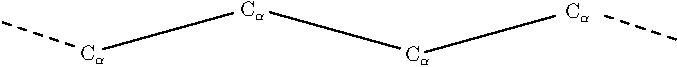
\includegraphics{Calpha_backbone}  
    \label{fig:Calpha_backbone}
  }
  \subbottom[The connection of amino acids in the protein backbone]{
    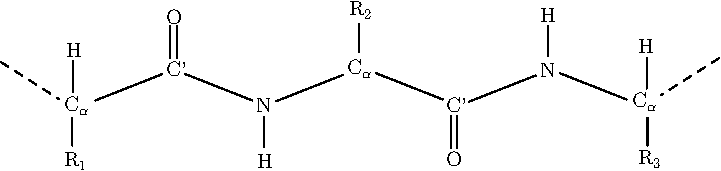
\includegraphics{amino_connect}  
    \label{fig:amino_connect}
  }
\end{figure}


The building stone of proteins are amino acids\footnote{A detailed
  introduction to the structure of proteins is found in
  \cite{branden}}. A protein consist of at least one linear chain of
amino acids. In Figure \ref{fig:amino_connect} we have shown how a
sequence of amino acids are connected. A carbon atom is located at the
center of each amino acid, this is called the $C_\alpha$ atom. The
largest variability of the protein structure is found in the angles
between the individual $C_\alpha$ atoms\cite{lotan04}, \textit{the torsion
angles}. Thus, the approach taken by the algorithms team at our
department is to describe the protein structure solely by the
$C_\alpha$ atoms, in the attempt to do protein structure prediction.

When a possible fold of a protein is found using this method, we will
add the missing atoms to construct a model of the complete protein,
including side chains. Apart from obtaining the position of all of the
atoms, we can use this to measure how well the backbone and side
chains fit together, and thereby get a more detailed indicator of how
accurate the backbone prediction is.

% Adding side chains to a folded backbone may
% introduce new problems. An added side chain can contribute with
% additional free energy, making the conformation unstable, and at worst
% causing collisions with other parts of the backbone or other side
% chains.

The stability of a protein is determined by the amount of free energy
in the structure. The goal of the protein structure prediction is thus
to find the most plausible protein structure by minimizing the free
energy. 
% Something here about how our addition of side chains can be used to
% determine the quality of their folding.

A realistic energy calculation will require an insight in
biochemistry that is beyond the scope of this project.  Therefore, we
limit ourselves to measure the sum of root mean square deviations,
RMSD, on the Euclidean distance between each atom of the true protein
structure and our structure prediction.



\section{Learning goals}
Our learning goals for this project includes:
\begin{itemize}
\item Models for representing protein structures and side-chains
\item Basics of protein structure prediction
% \item Apply linear algebra to represent rotations of protein structures
\item Apply transformations on three-dimensional protein models using linear algebra
\end{itemize}


\section{Limitations}
\begin{itemize}
\item Interconnections between side chain atoms from two different
  aminogroups, such as a disulfid-bridge between two side chains.
\item Energy computations
\end{itemize}

\bibliographystyle{apalike}
\bibliography{../bibliography}


% Spørgsmål til Rasmus:
%  - Energiberegning, Metropolis, Boltzmann etc.
%  - Leonard Jones potentialet

\end{document}

